\chapter{Introducción}\label{ch:Introducción}
Las epidemias han sido y son un problema que además de afectar a la salud pública, perjudican además otros aspectos
de la sociedad como la economía, la educación o la política. En la figura \ref{f:linea} podemos encontrar una línea temporal con algunas de las
principales pandemias o epidemias que han sucedido a lo largo de la historia.

\begin{figure}[H]
    \centering
    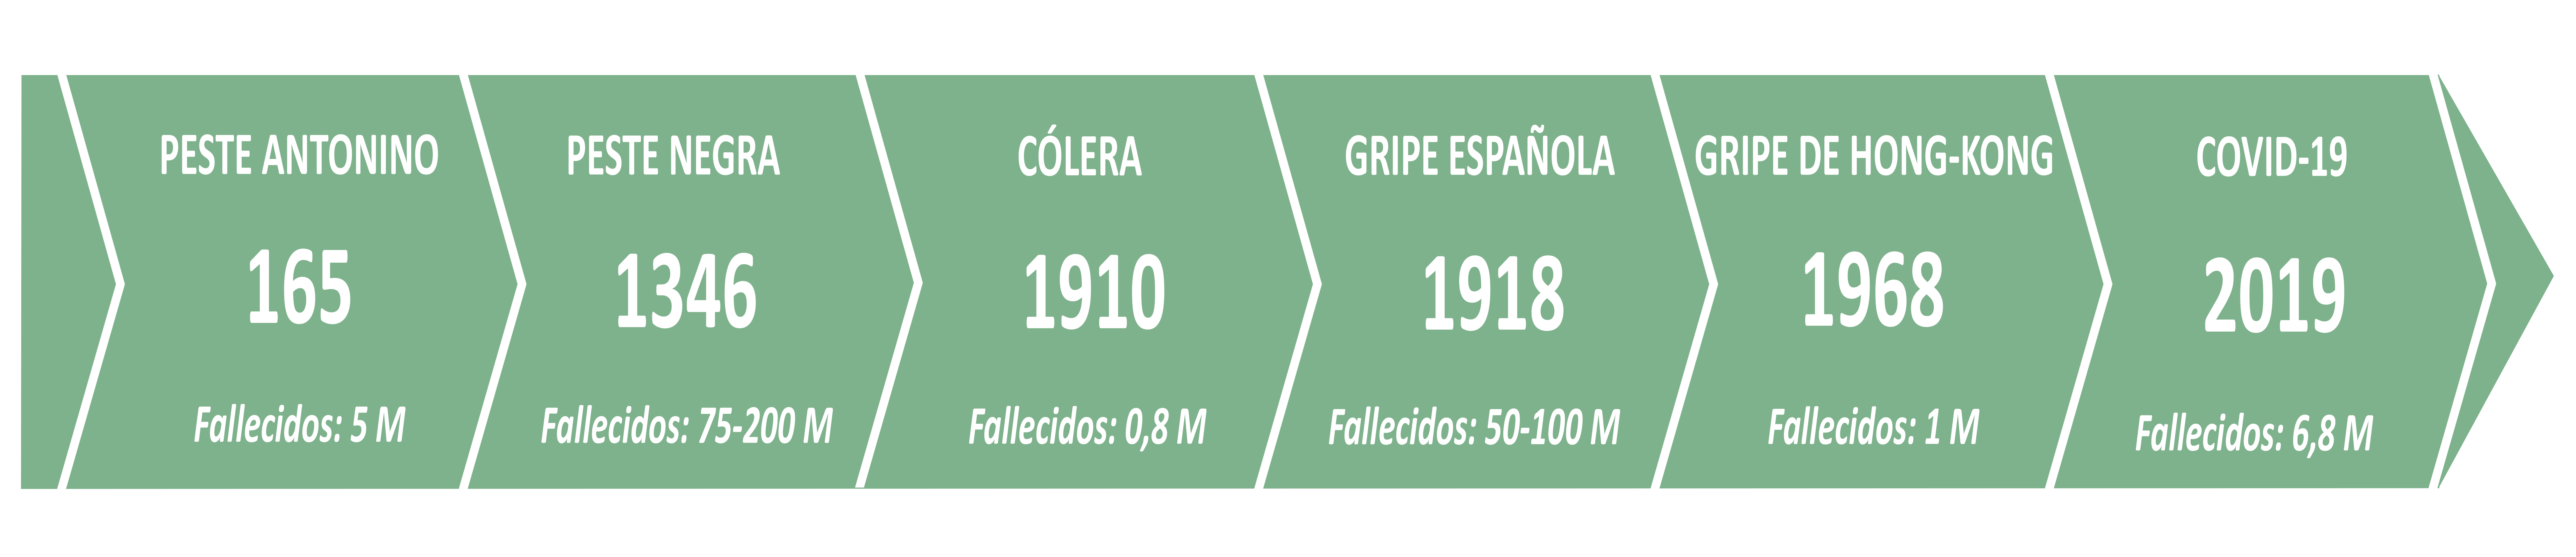
\includegraphics[width=0.75\textwidth]{Linea tiempo Antonio.png}
    \caption{Línea temporal con las principales pandemias, adaptado de los datos de la tabla 1 de \cite{castaneda2020principales}.}
    \label{f:linea}
\end{figure}

Por eso es importante entender como estas se transmiten, cómo podemos prevenir su expansión o controlarla 
en el caso en el que se haya producido la infección de una parte 
considerable de la población y así minimizar el impacto que tenga en la sociedad.
Para lograr entender el comportamiento de la expansión de las enfermedades, haremos uso de la 
física estadística como una herramienta para el estudio y modelado de estas. Podemos relacionar las epidemias con la física estadística, ya que tratamos a la población como un conjunto de partículas interaccionantes, 
al cual aplicaremos distintos modelos para pronosticar el comportamiento de la enfermedad. Tal y como hacemos con la física estadística,
estudiamos las interacciones microscópicas y a partir de estas obtenemos valores de magnitudes macroscópicas, lo que nos permitirá planificar diferentes
estrategias de prevención y control de esta. En este trabajo, nos centraremos en un modelo 
simple, el susceptible-infectado-susceptible (SIS) \cite{Chowell}. En este modelo encontramos dos posibles estados de los individuos,
infectado o susceptible a ser infectado. Los individuos infectados podrán pasar a ser susceptibles con cierta probabilidad por unidad de tiempo
y si un infectado interacciona con un susceptible podrá contagiarlo bajo otra probabilidad por unidad de tiempo. 

Para estudiar la evolución del sistema, utilizaremos el algoritmo de Gillespie \cite{Gillespie}, un algoritmo que nos permitirá obtener 
trayectorias compatibles con las soluciones de la ecuación maestra \cite{McKane,Toral}, una ecuación diferencial determinista para la 
probabilidad de encontrar a nuestro sistema en cierto estado discreto. Esta técnica tiene en cuenta la naturaleza estocástica 
e impredecible de las epidemias, debido a la incertidumbre probabilística de los contagios y recuperaciones. Además de usar método,
obtendremos la ecuación de Fokker-Planck \cite{McKane,Toral} a partir de la ecuación maestra, ya que es un desarrollo en serie a segundo orden 
de dicha ecuación, en este caso es una ecuación en derivadas parciales que nos permite obtener la probabilidad de encontrar nuestro sistema 
en cierto estado pero en este caso para una variable cuasicontinua, el número de infectados normalizado. Finalmente, partiendo de la ecuación 
de Fokker-Planck obtendremos la ecuación de Langevin \cite{McKane}, una ecuación diferencial estocástica para nuestra variable estocástica, 
el número de infectados normalizado. La resolución de esta ecuación también nos permitirá describir la evolución del sistema.

Para la resolución de dichas ecuaciones, debido a la complejidad o inexistencia de soluciones analíticas, recurriremos a resoluciones 
numéricas. Para ello, nos ayudaremos de los métodos Montecarlo \cite{kroese2014monte}, los cuales nos permiten resolver este tipo de problemas. Estos métodos
se basan en la generación de números aleatorios y repetición de cálculos para obtener una solución aproximada del problema. Además, nos 
permitirán predecir comportamientos de nuestro sistema de manera probabilística para poder estudiar los sistemas complejos.

A partir de la resolución de estas ecuaciones podremos obtener información cuantitativa sobre la propagación de la enfermedad, 
como la evolución temporal del número de infectados, la velocidad de transmisión, la probabilidad de que exista un brote epidémico. 
Distinguimos dos zonas en el problema, la zona absorbente y la zona activa. La primera se da cuando la velocidad de recuperación 
es mayor a la de infección, por lo que con el paso del tiempo, el número de individuos infectado es nulo. Por otro lado, nos encontramos en
la zona activa cuando la velocidad de infección es mayor que la de recuperación, por lo que el número de infectados con el paso del tiempo
no será nulo. Un brote epidémico cuando se produce con el paso de la zona absorbente a la activa, ya que la probabilidad de infección será 
mayor a la de recuperación y, por lo tanto, se producirá un aumento del número de infectados de la población.

Además, podemos usar la física estadística con otros aspectos de la vida. Por ejemplo, podemos comprender la propagación de información y rumores en redes sociales \cite{castellano2009statistical} 
o el contagio de comportamientos y opiniones. Los principios y enfoques utilizados para modelar las epidemias pueden ser aplicados
a una amplia gama de fenómenos sociales y biológicos \cite{azaele2016statistical} en los que la propagación 
y la interacción juegan un papel crucial.